\documentclass[twoside,twocolumn]{article}
\usepackage[hmarginratio=1:1,top=32mm,columnsep=20pt]{geometry}
\usepackage[hang, small,labelfont=bf,up,textfont=it,up]{caption}
\usepackage{amssymb} 
\usepackage{amsmath}
\usepackage{booktabs}
\usepackage{enumitem}
\setlist[itemize]{noitemsep}
\usepackage{abstract}
\renewcommand{\abstractnamefont}{\normalfont\bfseries}
\renewcommand{\abstracttextfont}{\normalfont\small\itshape}
\usepackage{titlesec}
\renewcommand\thesection{\Roman{section}}
\renewcommand\thesubsection{\Alph{subsection}}
\renewcommand\thesubsubsection{\arabic{subsubsection}}
\titleformat{\section}[block]{\normalsize\bfseries\scshape\centering}{\thesection.}{1em}{}
\titleformat{\subsection}[block]{\normalsize\bfseries\centering}{\thesubsection.}{1em}{}
\titleformat{\subsubsection}[block]{\normalsize\centering}{\thesubsubsection.}{1em}{}
\usepackage{fancyhdr}
\pagestyle{fancy}
\fancyhead{}
\fancyhead[C]{Computational Physics Homework $\bullet$ May 2018 $\bullet$ Vol. I, No. 5}
\usepackage{titling}
\usepackage{hyperref}
\hypersetup{unicode}
\AtBeginShipoutFirst{\input{zhwinfonts.tex}}
\usepackage{bm}
\usepackage{braket}
\usepackage{CJKutf8}
\usepackage{xcolor}
\usepackage{dcolumn}
\usepackage{graphicx}
\usepackage{indentfirst}
\usepackage{listings}
\usepackage[toc, page, title, titletoc, header]{appendix}
\definecolor{grey}{rgb}{0.8,0.8,0.8}
\definecolor{darkgreen}{rgb}{0,0.3,0}
\definecolor{darkblue}{rgb}{0,0,0.3}
\def\lstbasicfont{\fontfamily{pcr}\selectfont\footnotesize}
\lstset{
	numbers=left,
	numberstyle=\small,
	showstringspaces=false,
	showspaces=false,
	tabsize=4,
	frame=single,
	basicstyle={\footnotesize\lstbasicfont},
	keywordstyle=\color{darkblue}\bfseries,
	identifierstyle=,
	commentstyle=\color{darkgreen},
	stringstyle=\color{black}
}
\lstloadlanguages{C,C++,Fortran,Java,Matlab,Mathematica,Python}
\setlength{\parindent}{2em}
\begin{document}
\begin{CJK*}{UTF8}{gkai}
%----------------------------------------------------------------------------------------
%	TITLE SECTION
%----------------------------------------------------------------------------------------

\setlength{\droptitle}{-4\baselineskip} % Move the title up
\pretitle{\begin{center}\Huge\bfseries} % Article title formatting
	\posttitle{\end{center}} % Article title closing formatting
\title{计算物理第五次作业} % Article title
\author{
	\textsc{梁旭民}\thanks{\noindent 指导老师:齐新老师} \\[1ex] % Your name
	\normalsize Cuiying Hornors College, Lanzhou University \\ % Your institution
	\normalsize \href{mailto:liangxm15@lzu.edu.cn}{liangxm15@lzu.edu.cn} % Your email address
}
\date{}
\renewcommand{\maketitlehookd}{
	\begin{abstract}
		本次作业学习了Crank-Nicolson 差分格式求解含时微分方程的解法,并运用该方法求解了初始条件为Gauss函数的扩散方程,并画出了该扩散方程随时间的演化。
	\end{abstract}
}
\maketitle

%----------------------------------------------------------------------------------------
%	SECTION 1
%----------------------------------------------------------------------------------------

\section{第一个问题}
\subsection{问题描述}
已知一维扩散方程形式为
\begin{equation*}
\begin{aligned}
\frac{\partial u(x,t)}{\partial t}&=D\frac{\partial^{2}u(x,t)}{\partial x^{2}}\\
u(x,t)|_{t=0}&=u_{0}(x)\\
a_{1}u+b_{1}\frac{\partial u}{\partial n}&=c_{1}\quad (x=0)\\
a_{2}u+b_{2}\frac{\partial u}{\partial n}&=c_{2}\quad (x=a_{0})
\end{aligned}
\end{equation*}
例:考虑f=0,D=1,边界条件为$\phi(0)=\phi(1)=0$。设给定的初始条件是中心在$x=\frac{1}{2}$的一个Gauss函数,即:
\begin{equation*}
\phi(x,t=0)=\mathrm{e}^{-20(x-\frac{1}{2})^{2}}-\mathrm{e}^{-20(x-\frac{3}{2})^{2}}-\mathrm{e}^{-20(x+\frac{1}{2})^{2}}
\end{equation*}
求随后各个时刻的$\phi$。

若设$\tau=1+80t$,则解析解为:
\begin{equation*}
\phi(x,t)=\tau^{-\frac{1}{2}}[\mathrm{e}^{-20(x-\frac{1}{2})^{2}}-\mathrm{e}^{-20(x-\frac{3}{2})^{2}}-\mathrm{e}^{-20(x+\frac{1}{2})^{2}}]
\end{equation*}

上例可以用标准的Crank-Nicolson方法求解。
\subsection{问题分析}
Crank-Nicolson是一种数值分析的有限差分法,可用于数值求解热方程以及类似形式的偏微分方程[2]。它在时间方向上是隐式的二阶方法,可以写成隐式的Runge-Kutta法,数值稳定。该方法诞生于20世纪,由John Crank与Phyllis Nicolson发展[3]。

可以证明Crank-Nicolson方法对于扩散方程(以及许多其他方程)是无条件稳定[4]。但是,如果时间步长$\Delta t$乘以热扩散率,再除以空间步长平方$\Delta t^{2}$的值过大(根据Von Neumann稳定性分析,以大于$\frac{1}{2}$为准),近似解中将存在虚假的振荡或衰减。基于这个原因,当要求大时间步或高空间分辨率的时候,往往会采用数值精确较差的后向欧拉法进行计算,这样即可以保证稳定,又避免了解的伪振荡。
\subsubsection{一维扩散方程Crank-Nicolson格式}
已知一维扩散方程形式为
\begin{equation*}
\left\{
\begin{aligned}
&\frac{\partial u(x,t)}{\partial t}=D\frac{\partial^{2}u(x,t)}{\partial x^{2}}\\
&\left.u(x,t)\right|_{t=0}=u_{0}(x)\\
&a_{1}u+b_{1}\frac{\partial u}{\partial n}=c_{1}\qquad (x=0)\\
&a_{2}u+b_{2}\frac{\partial u}{\partial n}=c_{2}\qquad (x=a_{0})
\end{aligned}
\right.
\end{equation*}
取$\Delta x=h,\Delta t=\tau$进行离散化,节点坐标为
\begin{equation*}
\left\{
\begin{aligned}
&x_{i}=(i-1)h\qquad (i=1,2,...,N)\\
&t_{k}=k\tau\qquad (k=1,2,...,k_{max})
\end{aligned}
\right.
\end{equation*}
\begin{figure}[h]
	\centering
	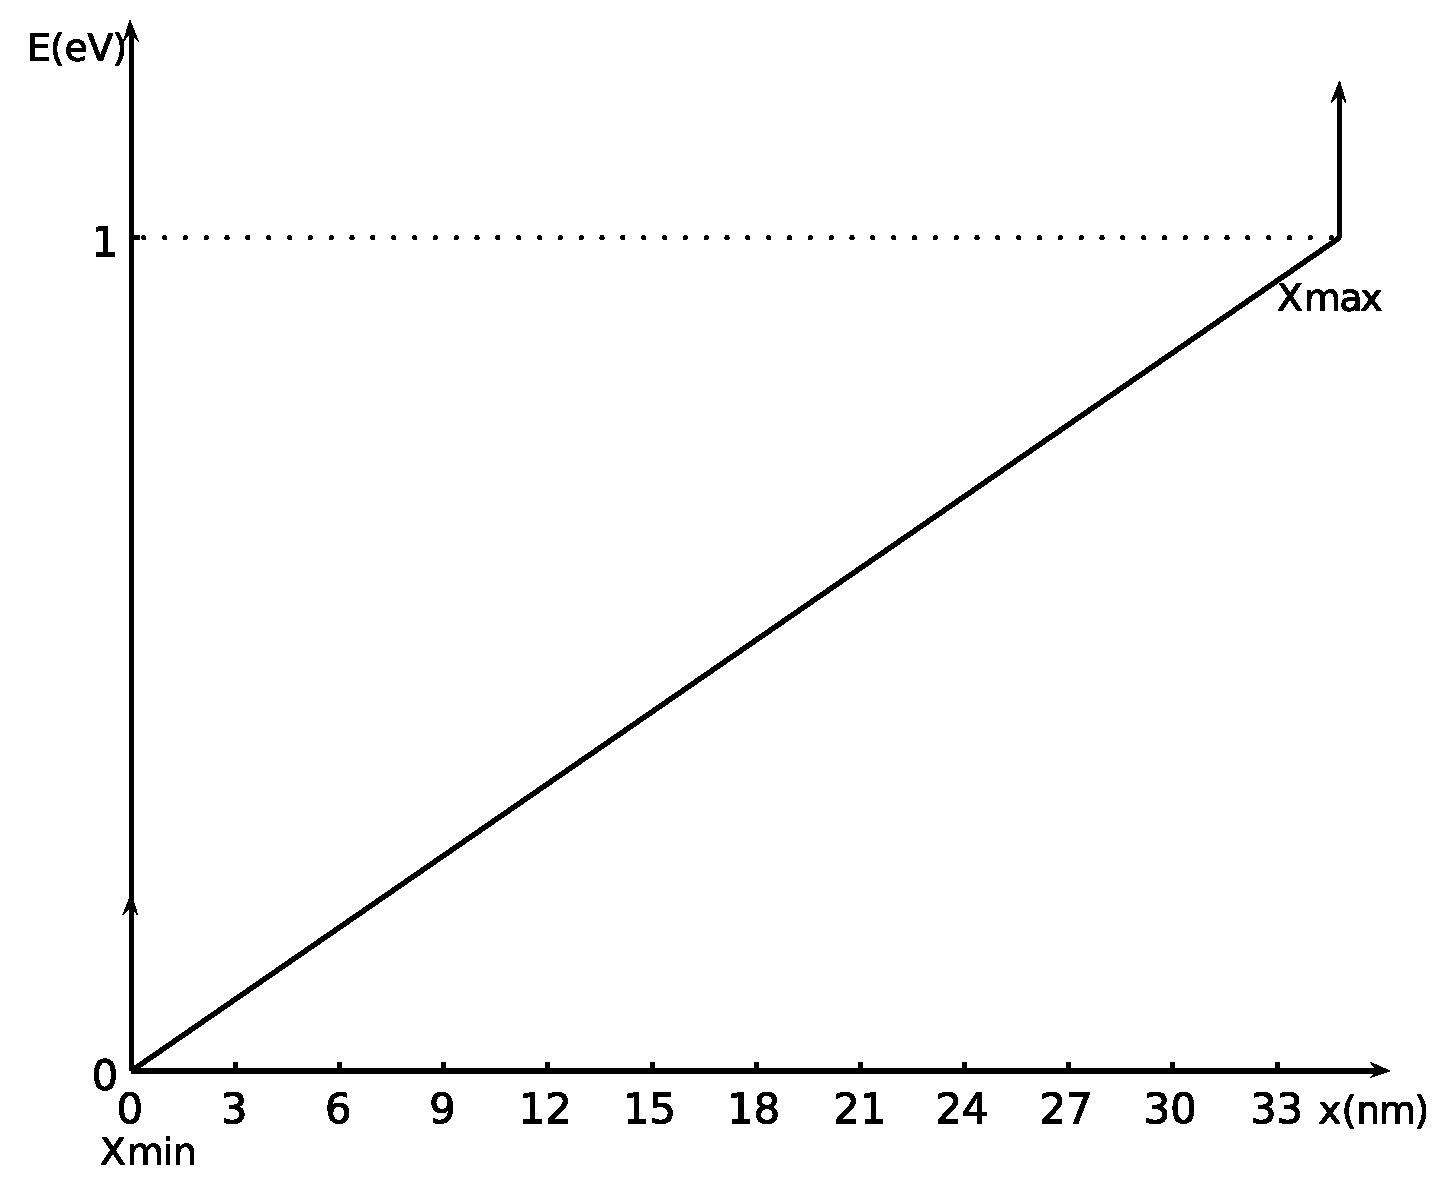
\includegraphics[width=1.0\linewidth]{figure/fig1}
	\caption{一维扩散方程的隐式六点差分格式}
	\label{fig:fig1}
\end{figure}

节点处的函数为
\begin{equation*}
u(x-{i},t_{k})=u_{i}^{k}
\end{equation*}
利用如下差分格式
\begin{equation*}
\begin{aligned}
&f^{\prime}(0)\approx \frac{f_{1}-f_{-1}}{2h}\\
&\frac{\partial u}{\partial t}=\frac{u_{i}^{k+1}-u_{i}^{k}}{\tau}\\
&\frac{\partial^{2}u}{\partial x^{2}}=\frac{1}{2}\left[\left(\frac{u_{i+1}-2u_{i}+u_{i-1}}{h^{2}}\right)^{k}\right.\\
&\left.+\left(\frac{u_{i+1}-2u_{i}+u_{i-1}}{h^{2}}\right)^{k+1}\right]\\
&\frac{u_{i}^{k+1}-u_{i}^{k}}{\tau}=\frac{D}{2h^{2}}\left[\left(u_{i+1}-2u_{i}+u_{i-1}\right)^{k}\right.\\
&\left.+\left(u_{i+1}-2u_{i}+u_{i-1}\right)^{k+1}\right]
\end{aligned}
\end{equation*}

令$P=\frac{\tau D}{h^{2}},P_{1}=\frac{1}{P}+1,P_{2}=\frac{1}{P}-1$,则可以得到隐式六点差分格式(Crank-Nicolson格式)
\begin{equation*}
\begin{aligned}
&\left(-u_{i-1}+2P_{1}u_{i+1}-u_{i+1}\right)^{k+1}\\
&=\left(u_{i-1}+2P_{2}u_{i}+u_{i+1}\right)^{k}
\end{aligned}
\end{equation*}
\subsubsection{边界条件的处理}
\begin{equation*}
\left\{
\begin{aligned}
&a_{1}u+b_{1}\frac{\partial u}{\partial n}=c_{1}\qquad (x=0)\\
&a_{2}u+b_{2}\frac{\partial u}{\partial n}=c_{2}\qquad (x=a_{0})
\end{aligned}
\right.
\end{equation*}
\begin{figure}[h]
\centering
\includegraphics[width=1.0\linewidth]{figure/fig2}
\caption{1维扩散方程的边界条件}
\label{fig:fig2}
\end{figure}

设置虚格点$i=0,i=N+1$,利用中心差商公式有
\begin{equation*}
\left\{
\begin{aligned}
&a_{1}u_{1}+b_{1}\frac{u_{0}-u_{2}}{2h}=c_{1}\qquad &(x=0)\\
&a_{2}u_{n}+b_{2}\frac{u_{n+1}-u_{n-1}}{2h}=c_{2}\qquad &(x=a_{0})
\end{aligned}
\right.
\end{equation*}

解出$u_{0},u_{n+1}$代入$i=1,i=N$的Crank-Nicolson差分格式
\begin{equation*}
\begin{aligned}
&\left[\left(b_{1}P_{1}+ha_{1}\right)u_{1}-b_{1}u_{2}\right]^{k+1}\\
&=\left[\left(b_{1}P_{2}-ha_{1}\right)u_{1}+b_{1}u_{2}\right]^{k}+2hc_{1}\\
&\left[-b_{2}u_{N-1}+\left(b_{2}P_{1}+ha_{2}\right)u_{N}\right]^{k+1}\\
&=\left[b_{2}u_{N-1}+\left(b_{2}P_{2}-ha_{2}\right)u_{N}\right]^{k}+2hc_{2}
\end{aligned}
\end{equation*}

差分方程组及其求解:

将上述差分公式和边界条件结合起来,得到差分线性方程组,其形式为:
\begin{equation*}
\mathbf{AU}=\mathbf{R}
\end{equation*}
其中,\\
$\mathbf{U}=(u_{1},u_{2},...,u_{n})$是未知量组成的矢量。\\
$\mathbf{R}=(R_{1},R_{2},...,R_{n})$是有前一时刻的u值组成的矢量。\\

则有
\begin{equation*}
\begin{aligned}
&R_{1}=(b_{1}P_{2}-ha_{1})u_{1}+b_{1}u_{2}+2hc_{1}\\
&R_{i}=u_{i-1}+2P_{2}u_{i}+u_{i+1}\qquad i=2,3,...,N-1\\
&R_{N}=b_{2}u_{N-1}+(b_{2}P_{2}-ha_{2})u_{N}+2hc_{2}
\end{aligned}
\end{equation*}
系数矩阵A是三对角的
\begin{equation*}
\begin{bmatrix} 
b_ {1}P_{1}+ha_{1}&-b_{1}&0&\cdots&0&0\\
-1&2P_{1}&-1&0&\cdots&0\\
0&-1&2P_{1}&-1&\ddots&\vdots\\
\vdots&\ddots&\ddots&\ddots&\ddots&\vdots\\
\vdots&\ddots&-1&2P_{1}&-1&0\\
0&\cdots&0&-1&2P_{1}&-1\\
0&0&\cdots&0&-b_{2}&b_{2}P_{1}+ha_{2}
\end{bmatrix}
\end{equation*}

这是一个三对角问题,应用追赶法即可得到$u_{i}^{k+1}$,而不需要对矩阵直接求逆。
\subsection{计算结果}
运行结果见压缩包中的figure文件夹中的动画1dDiffusion.gif,以下只展示截图
\begin{figure}[h]
	\centering
	\includegraphics[width=1.0\linewidth]{figure/1dDiffusion/_tmp00000}
	\caption{1维扩散方程瞬时截图}
\end{figure}
\newpage
\section{第二个问题}
\subsection{问题表述}
试将第一个问题拓展成二维,求解二维扩散方程随时间的演化并画图(初始条件、边界条件自设,你可以选择二维Crank-Nicolson方法,也可以选择简单Eular法,也可以选择上一章提到的迭代法)。
\subsection{问题分析}
\subsubsection{二维扩散方程}
将扩散问题延伸到二维的Cartesian网络,我们有类似的推导:

二维的扩散方程形式为
\begin{equation*}
\left\{
\begin{aligned}
&\frac{\partial u}{\partial t}=D\left({\frac{\partial ^{2}u}{\partial x^{2}}}+{\frac{\partial^{2}u}{\partial y^{2}}}\right)\qquad
\left(
\begin{aligned}
&0<x<a_{0}\\&0<y<b_{0}\\&0<t<t_{max}
\end{aligned}\right)\\
&u(x,y,0)=u_{0}(x,y)
\end{aligned}\right.
\end{equation*}
取$\Delta x=\Delta y=h$的正方形网格覆盖x-y平面,并取$\Delta t=\tau$,节点坐标为
\begin{equation*}
\left\{
\begin{aligned}
&x_{i}=(i-1)h\qquad (i=1,2,\cdots ,N)\\
&y_{i}=(i-1)h\qquad (j=1,2,\cdots ,M)\\
&t_{k}=k\tau\qquad (k=1,2,\cdots ,k_{max})
\end{aligned}
\right.
\end{equation*}
节点处的函数为$u(x_{i},y_{j},t_{k})=u_{ij}^{k}$

在$(i,j,k+\frac{1}{2})$点,将$\frac{\partial u}{\partial t}$用$k$时中心差商代替,将$\frac{\partial^{2}u}{\partial x^{2}}$用$k+1$时的中心差商代替,将$\frac{\partial^{2} u}{\partial y^{2}}$用$k$时的中心差商代替,则二维扩散方程变为
\begin{equation*}
\begin{aligned}
&\frac{u_{ij}^{k+1}-u_{ij}^{k}}{\tau}=\frac{D}{h^{2}}[\left(u_{i+1,j}-2u_{ij}+u_{i-1,j}\right)^{k+1}\\
&+\left(u_{i,j+1}-2u_{ij}+u_{i,j-1}\right)^{k}]
\end{aligned}
\end{equation*}

在$(i,j,k+\frac{3}{2})$点,将$\frac{\partial u}{\partial t}$用$k+1$时中心差商代替,将$\frac{\partial^{2}u}{\partial x^{2}}$用$k+1$时的中心差商代替,将$\frac{\partial^{2} u}{\partial y^{2}}$用$k+2$时的中心差商代替,则二维扩散方程变为
\begin{equation*}
\begin{aligned}
&\frac{u_{ij}^{k+2}-u_{ij}^{k+1}}{\tau}=\frac{D}{h^{2}}[\left(u_{i+1,j}-2u_{ij}+u_{i-1,j}\right)^{k+1}\\
&+\left(u_{i,j+1}-2u_{ij}+u_{i,j-1}\right)^{k+2}]
\end{aligned}
\end{equation*}

令$P=\frac{\tau D}{h^{2}},P_{1}=\frac{1}{P}+1,P_{2}=\frac{1}{P}-1$,则有
\begin{equation*}
\begin{aligned}
&(-u_{i-1,j}+2P_{1}u_{ij}-u_{i+1,j})^{k+1}\\
&=(u_{i,j-1}+2P_{2}u_{ij}+u_{i,j+1})^{k}\qquad\quad \cdots (a)\\
&(-u_{i-1,j}+2P_{1}u_{ij}-u_{i+1,j})^{k+2}\\
&=(u_{i,j-1}+2P_{2}u_{ij}+u_{i+1,j})^{k+1}\qquad \cdots (b)
\end{aligned}
\end{equation*}
说明:\\
1.求解方法与一维情形类似。\\
2.k为奇数时用(b)式沿y方向计算,k为偶数时用(a)式沿x方向计算,并且只输出后一结果,以减少因为时间上的不一致引起的误差。\\
3.该方法是无条件稳定的。\\
\subsubsection{边界条件的处理}
边界条件的差分格式\\
\begin{equation*}
\left\{
\begin{aligned}
&a_{i}u+b_{i}\frac{\partial u}{\partial n}=c_{i}(y,t)\qquad (1)(2)\text{边界}(i=1,2)\\
&a_{i}u+b_{i}\frac{\partial u}{\partial n}=c_{i}(x,t)\qquad (3)(4)\text{边界}(i=3,4)
\end{aligned}
\right.
\end{equation*}
\begin{figure}[h]
	\centering
	\includegraphics[width=0.6\linewidth]{figure/fig3}
	\caption{2维扩散方程边界条件}
	\label{fig:fig3}
\end{figure}

设置虚节点:\\
在(1)(2)边界上有
\begin{equation*}
\left\{
\begin{aligned}
&b_{1}u_{0j}=2hc_{1}(y_{i},t)-2ha_{1}u_{1j}+b_{1}u_{2j}~~~~~~~~~~(1)\\
&b_{2}u_{n+1,j}=2hc_{2}(y_{i},t)-2ha_{1}u_{nj}+b_{2}u_{n-1,j}~~(2)
\end{aligned}
\right.
\end{equation*}
在(3)(4)边界上有
\begin{equation*}
\left\{
\begin{aligned}
&b_{3}u_{i0}=2hc_{3}(x_{i},t)-2ha_{3}u_{i1}+b_{3}u_{i2}~~~~~~~~~~~(3)\\
&b_{4}u_{i,m+1}=2hc_{4}(x_{i},t)-2ha_{4}u_{im}+b_{4}u_{i,m-1}~(4)
\end{aligned}
\right.
\end{equation*}

解出$u_{i0},u_{i,m+1}$
结果会是带形矩阵的方程式。
\subsection{计算结果}
运行结果见压缩包中的figure文件夹中的动画2dDiffusion.mp4,以下只展示截图
\begin{figure}[h]
\centering
\includegraphics[width=1.0\linewidth]{figure/fig5}
\caption{2维扩散方程动画瞬时截图}
\label{fig:fig5}
\end{figure}

%----------------------------------------------------------------------------------------
%	APPENDICES SECTION
%----------------------------------------------------------------------------------------

\newpage
\onecolumn
\begin{appendices}
\section{使用Crank-Nicolson方法求解一维扩散方程}
Here is the program to solve the one dimensional diffusion equation by Crank-Nicolson method in Python programming language.\\
\textbf{\textcolor[rgb]{0.98,0.00,0.00}{Input Python source:}}
\lstinputlisting[language=Python]{./program/1D_Diffusion.py}
\section{一维扩散方程动画}
Here is the program to merge png pictures together to gif animation in Python programming language.\\
\textbf{\textcolor[rgb]{0.98,0.00,0.00}{Input Python source:}}
\lstinputlisting[language=Python]{./program/merge.py}
\section{求解二维扩散方程}
Here is the program to two dimensional diffusion equation in Python programming language.\\
\textbf{\textcolor[rgb]{0.98,0.00,0.00}{Input Python source:}}
\lstinputlisting[language=Python]{./program/2D_Diffusion.py}	
\end{appendices}

%----------------------------------------------------------------------------------------
%	REFERENCE
%----------------------------------------------------------------------------------------

\newpage
\renewcommand\refname{参考文献}
\begin{thebibliography}{99}
	\bibitem{ref1}Tuncer Cebeci. Convective Heat Transfer. Springer. 2002. ISBN 0-9668461-4-1.
	\bibitem{ref2}Crank, J.; Nicolson, P. A practical method for numerical evaluation of solutions of partial differential equations of the heat conduction type. Proc. Camb. Phil. Soc. 1947, 43 (1): 50–67. doi:10.1007/BF02127704.
	\bibitem{ref3} Thomas, J. W. Numerical Partial Differential Equations: Finite Difference Methods. Texts in Applied Mathematics 22. Berlin, New York: Springer-Verlag. 1995. ISBN 978-0-387-97999-1.. Example 3.3.2 shows that Crank–Nicolson is unconditionally stable when applied to$u_{t}=au_{xx}$
	\bibitem{ref4}Wilmott, P.; Howison, S.; Dewynne, J. The Mathematics of Financial Derivatives: A Student Introduction. Cambridge Univ. Press. 1995. ISBN 0-521-49789-2.
\end{thebibliography} 

%----------------------------------------------------------------------------------------
\end{CJK*}
\end{document}
